\documentclass[12pt, a4paper]{article}

% Margins and Geometry
\usepackage[margin=1in]{geometry}

% Input Encoding
\usepackage[utf8]{inputenc}

% Math and Symbols
\usepackage{amsmath, amssymb}

% Graphics and Colors
\usepackage{tikz}
\usetikzlibrary{shapes, arrows.meta, positioning}
\usepackage{graphicx}
\usepackage[dvipsnames,table]{xcolor} % Using more color names, enable table features

% Tables
\usepackage{booktabs} % For professional looking tables
\usepackage{array} % For better column definitions
\usepackage{makecell} % Allows line breaks in cells

% Layout and Formatting
\usepackage{fancyhdr} % For headers and footers
\usepackage{titlesec} % To customize section titles
\usepackage{caption} % For captions outside floats
\usepackage{multicol} % For multi-column layout (optional)
\usepackage{parskip} % Adds space between paragraphs instead of indent

% Icons (Using fontawesome5 for more icons)
\usepackage{fontawesome5}

% Code Listing
\usepackage{listings} % For code blocks
\usepackage{tcolorbox} % For colored boxes around text/code
\tcbuselibrary{listings, skins, breakable} % Integrate tcolorbox with listings, skins and allow breaking

% Hyperlinks (Optional, but good for references)
% Load hyperref last with few exceptions (like cleveref)
\usepackage[hidelinks]{hyperref}


%-------------------------------------------------------------------------------
% Customization
%-------------------------------------------------------------------------------

% Page Style
\pagestyle{fancy}
\fancyhf{} % Clear header/footer
\lhead{\textcolor{RoyalBlue}{\faBookOpen~ Graphics Notes}}
\rhead{\textcolor{RoyalBlue}{\faDotCircle~ Bresenham's Circle Algorithm}}
\cfoot{\textcolor{gray}{Page \thepage}}
\renewcommand{\headrulewidth}{0.4pt} % Header rule
\renewcommand{\footrulewidth}{0.4pt} % Footer rule

% Section Title Formatting
\titleformat{\section}
  {\Large\bfseries\color{NavyBlue}} % Format
  {\color{NavyBlue}\faAngleRight~\thesection.} % Label
  {0.5em} % Horizontal separation
  {} % Code before title
  [\color{NavyBlue}\titlerule] % Code after title (adds a rule)

\titleformat{\subsection}
  {\large\bfseries\color{MidnightBlue}} % Format
  {\color{MidnightBlue}\faCaretRight~\thesubsection.} % Label
  {0.5em} % Horizontal separation
  {} % Code before title

% TikZ Style
\tikzstyle{point}=[circle, fill=blue, inner sep=1.5pt]
\tikzstyle{centerpoint}=[circle, fill=red, inner sep=1.5pt]
\tikzstyle{axis}=[->, >=Latex, thick, gray]
\tikzstyle{gridline}=[thin, gray!40]
\tikzstyle{dashedcircle}=[dashed, gray]

% Listings Style (for code blocks)
\lstdefinestyle{customcpp}{
  language=C++,
  basicstyle=\ttfamily\small,
  keywordstyle=\color{blue}\bfseries,
  stringstyle=\color{purple},
  commentstyle=\color{ForestGreen}\itshape,
  numbers=left,
  numberstyle=\tiny\color{gray},
  stepnumber=1,
  numbersep=5pt,
  backgroundcolor=\color{gray!10},
  showspaces=false,
  showstringspaces=false,
  showtabs=false,
  frame=tb, % Top and bottom frame
  framerule=0pt, % Frame rule width
  captionpos=b, % Caption position
  breaklines=true,
  breakatwhitespace=true,
  tabsize=2,
  morekeywords={uint32_t, GL_POINTS, glBegin, glEnd, glVertex2i} % Add OpenGL specific keywords
}

\lstdefinestyle{custompy}{
  language=Python,
  basicstyle=\ttfamily\small,
  keywordstyle=\color{blue}\bfseries,
  stringstyle=\color{purple},
  commentstyle=\color{ForestGreen}\itshape,
  numbers=left,
  numberstyle=\tiny\color{gray},
  stepnumber=1,
  numbersep=5pt,
  backgroundcolor=\color{gray!10},
  showspaces=false,
  showstringspaces=false,
  showtabs=false,
  frame=tb,
  framerule=0pt,
  captionpos=b,
  breaklines=true,
  breakatwhitespace=true,
  tabsize=2,
}

% tcolorbox setup for code
\newtcblisting{cppcode}{
  listing engine=listings,
  listing only,
  breakable, % Allows the box to break across pages
  colback=gray!5,
  colframe=NavyBlue!75!black,
  title=\faCode~ C++ / OpenGL Implementation Snippet,
  fonttitle=\bfseries,
  listing options={style=customcpp},
  enhanced,
  overlay={\draw[NavyBlue!75!black,line width=0.5pt] ([yshift=-2pt]frame.south west)--([yshift=-2pt]frame.south east);} % Manual bottom rule inside box
}

\newtcblisting{pythoncode}{
  listing engine=listings,
  listing only,
  breakable, % Allows the box to break across pages
  colback=gray!5,
  colframe=OliveGreen!75!black,
  title=\faPython~ Python Implementation Snippet,
  fonttitle=\bfseries,
  listing options={style=custompy},
  enhanced,
  overlay={\draw[OliveGreen!75!black,line width=0.5pt] ([yshift=-2pt]frame.south west)--([yshift=-2pt]frame.south east);} % Manual bottom rule inside box
}

% Custom command for drawing symmetric points in TikZ
\newcommand{\drawCirclePoints}[2]{
    \node[point] at (#1,#2) {}; \node[point] at (#2,#1) {};
    \node[point] at (-#1,#2) {}; \node[point] at (-#2,#1) {};
    \node[point] at (#1,-#2) {}; \node[point] at (#2,-#1) {};
    \node[point] at (-#1,-#2) {}; \node[point] at (-#2,-#1) {};
}

% Increase row spacing slightly for makecell
\renewcommand{\arraystretch}{1.3}
% Set default alignment for makecell to left
\setcellgapes{3pt} % Add a little padding within cells
\makegapedcells % Apply the gapes

%-------------------------------------------------------------------------------
% Document Start
%-------------------------------------------------------------------------------
\begin{document}

% Title Block
\begin{tcolorbox}[
    colback=RoyalBlue!10!white,
    colframe=RoyalBlue!75!black,
    sharp corners,
    boxrule=1pt,
    center title
    ]
    {\Huge \bfseries \faDotCircle~ Bresenham's Circle Drawing Algorithm} \\[0.2cm]
    {\large A Structured Study Note with Code Examples}
\end{tcolorbox}
\vspace{0.5cm}

% Quick Notes Section
\begin{tcolorbox}[
    colback=yellow!10!white,
    colframe=orange!75!black,
    title=\faStickyNote~ Quick Notes,
    fonttitle=\bfseries\large
    ]
    \begin{itemize}
        \item An efficient algorithm for drawing circles on raster displays (pixel grids).
        \item Uses only \textbf{integer arithmetic} (addition, subtraction, bit-shifting), avoiding costly floating-point operations and square roots.
        \item Exploits \textbf{8-way symmetry}: calculates points for one octant (45-degree segment) and reflects them to get the full circle.
        \item Incremental calculation: determines the next pixel based on a decision parameter derived from the circle equation.
    \end{itemize}
\end{tcolorbox}

\section{Initial Setup}
We start by defining the circle's properties and the initial parameters for the algorithm. We focus on the second octant (from 90 to 45 degrees) and start at the top point of the circle.
\begin{itemize}
    \item Circle Center $(x_c, y_c) = (0, 0)$ (For simplicity; can be translated later)
    \item Radius $R$
    \item Starting Point: $(x_0, y_0) = (0, R)$
    \item Initial Decision Parameter $p_0$: Derived from evaluating the circle equation $f(x, y) = x^2 + y^2 - R^2$ at the midpoint between the two potential next pixels $(1, R)$ and $(1, R-1)$. The midpoint is $(1, R - 0.5)$.
    \[
        p_0 = f(1, R - 0.5) = 1^2 + (R - 0.5)^2 - R^2 = 1 + R^2 - R + 0.25 - R^2 = 1.25 - R
    \]
    To avoid fractions, we can use an integer-only version: $p_0 = 4 \times (1.25 - R) = 5 - 4R$.
    \textit{(Note: Sometimes $p_0 = 3 - 2R$ is used, derived differently but leading to equivalent update rules with adjustments.)} Let's use $p_0 = 3 - 2R$ for consistency with the original example.
    \item \textbf{Example:} For $R = 5$:
    \[
        p_0 = 3 - 2 \times 5 = 3 - 10 = -7
    \]
\end{itemize}

\section{Decision Parameter and Update Rules}
At each step $k$, starting with $(x_k, y_k)$, we decide whether the next point $(x_{k+1}, y_{k+1})$ is $(x_k+1, y_k)$ (move East) or $(x_k+1, y_k-1)$ (move South-East). This decision is based on the sign of the decision parameter $p_k$.

\begin{center}
\captionof{table}{Update Rules Based on Decision Parameter $p_k$}
\label{tab:update_rules}
% Using makecell for headers and adjusted column types
% Using 'l' for left-alignment where text wrapping might occur
\begin{tabular}{@{}c l c l@{}}
\toprule
% Headers using makecell for potential wrapping
\textbf{Condition} & \makecell[l]{\textbf{Next Pixel}\\\textbf{Choice}} & \makecell[c]{\textbf{Next Point}\\\textbf{$(x_{k+1}, y_{k+1})$}} & \makecell[l]{\textbf{Update Rule}\\\textbf{for } $p_{k+1}$} \\
\midrule
% Content row 1 - Update Rule content is in the last column
$p_k < 0$ & \makecell[l]{Pixel $(x_k+1, y_k)$ \\ is closer} & $(x_k+1, y_k)$ & $p_{k+1} = p_k + 4x_k + 6$ \\
\midrule % Rule between rows
% Content row 2 - Update Rule content is in the last column
$p_k \geq 0$ & \makecell[l]{Pixel $(x_k+1, y_k-1)$ \\ is closer} & $(x_k+1, y_k-1)$ & $p_{k+1} = p_k + 4(x_k - y_k) + 10$ \\
\bottomrule
\end{tabular}
\end{center}
The calculation stops when $x \geq y$, as this marks the end of the second octant.

\section{Step-by-Step Calculation (Example: R=5)}
\textbf{Given:} $R = 5$, Center $(0, 0)$, Start Point $(0, 5)$, $p_0 = -7$.

\begin{center}
\captionof{table}{Calculation steps for R=5 using the specified update rules.}
\label{tab:calc_steps}
% Using makecell for headers to allow wrapping
\begin{tabular}{|c|c|c|c|c|l|}
\hline
% Headers using makecell for potential wrapping
\makecell{\textbf{Step}\\\textbf{(k)}} & \makecell[c]{\textbf{Current Point}\\\textbf{$(x_k, y_k)$}} & $p_k$ & \makecell{\textbf{$p_k < 0$?}} & \makecell[c]{\textbf{Next Point}\\\textbf{$(x_{k+1}, y_{k+1})$}} & \makecell[l]{\textbf{Calculation}\\\textbf{for } $p_{k+1}$} \\
\hline
% Content rows using makecell for the last column
0 & (0, 5) & -7 & Yes & (1, 5) & \makecell[l]{$p_1 = p_0 + 4x_0 + 6$ \\ $= -7 + 4(0) + 6 = -1$} \\
\hline
1 & (1, 5) & -1 & Yes & (2, 5) & \makecell[l]{$p_2 = p_1 + 4x_1 + 6$ \\ $= -1 + 4(1) + 6 = 9$} \\
\hline
2 & (2, 5) & 9 & No & (3, 4) & \makecell[l]{$p_3 = p_2 + 4(x_2 - y_2) + 10$ \\ $= 9 + 4(2 - 5) + 10$ \\ $= 9 - 12 + 10 = 7$} \\
\hline
3 & (3, 4) & 7 & No & (4, 3) & \makecell[l]{$p_4 = p_3 + 4(x_3 - y_3) + 10$ \\ $= 7 + 4(3 - 4) + 10$ \\ $= 7 - 4 + 10 = 13$} \\
\hline
\multicolumn{6}{|c|}{\textbf{Stop:} $x=4, y=3 \implies x > y$} \\
\hline
\end{tabular}
\end{center}

The points generated in the second octant are: $(0, 5), (1, 5), (2, 5), (3, 4), (4, 3)$.
\textit{(Note: The previous calculation in the prompt stopped early and had slightly different intermediate values, likely due to using $p_k + 4(x+1) + 6$ instead of $p_k + 4x_k + 6$. The rules in Table \ref{tab:update_rules} are standard.)}

\section{Exploiting 8-Way Symmetry}
The core strength of Bresenham's circle algorithm is calculating points for only one 45-degree segment (an octant) and then reflecting these points across the axes and diagonals ($y=x, y=-x$) to obtain the full circle. If $(x, y)$ is a point calculated in the primary octant (e.g., the one from $x=0$ to $x=y$), the following points are also on the circle:

\begin{center}
\captionof{table}{Mapping a Point $(x, y)$ to All 8 Octants}
\label{tab:symmetry}
\rowcolors{2}{gray!15}{white} % Alternating row colors
\begin{tabular}{ccc}
\toprule
\textbf{Octant} & \textbf{Symmetric Point} & \textbf{Transformation from (x, y)} \\
\midrule
1 ($0^\circ-45^\circ$) & $(y, x)$ & Swap x and y \\
2 ($45^\circ-90^\circ$) & $(x, y)$ & Original point (calculated) \\
3 ($90^\circ-135^\circ$) & $(-x, y)$ & Negate x \\
4 ($135^\circ-180^\circ$) & $(-y, x)$ & Swap x and y, negate new x \\
5 ($180^\circ-225^\circ$) & $(-y, -x)$ & Swap x and y, negate both \\
6 ($225^\circ-270^\circ$) & $(-x, -y)$ & Negate both \\
7 ($270^\circ-315^\circ$) & $(x, -y)$ & Negate y \\
8 ($315^\circ-360^\circ$) & $(y, -x)$ & Swap x and y, negate new y \\
\bottomrule
\end{tabular}
\end{center}

\textbf{Applying Symmetry to R=5 Example Points:}\\
The calculated points were $(0, 5), (1, 5), (2, 5), (3, 4), (4, 3)$.
Using the symmetry rules:
\begin{itemize}
    \item From (0, 5): (5, 0), (0, 5), (0, 5), (-5, 0), (-5, 0), (0, -5), (0, -5), (5, 0) $\rightarrow$ Unique: $(\pm 5, 0), (0, \pm 5)$
    \item From (1, 5): (5, 1), (1, 5), (-1, 5), (-5, 1), (-5, -1), (-1, -5), (1, -5), (5, -1)
    \item From (2, 5): (5, 2), (2, 5), (-2, 5), (-5, 2), (-5, -2), (-2, -5), (2, -5), (5, -2)
    \item From (3, 4): (4, 3), (3, 4), (-3, 4), (-4, 3), (-4, -3), (-3, -4), (3, -4), (4, -3)
    \item From (4, 3): (3, 4), (4, 3), (-4, 3), (-3, 4), (-3, -4), (-4, -3), (4, -3), (3, -4) \textit{(Note: (3,4) and (4,3) generate the same set due to symmetry around y=x)}
\end{itemize}
These points, when plotted relative to the center $(x_c, y_c)$, form the complete circle.

\section{Visualization (TikZ)}

\begin{center}
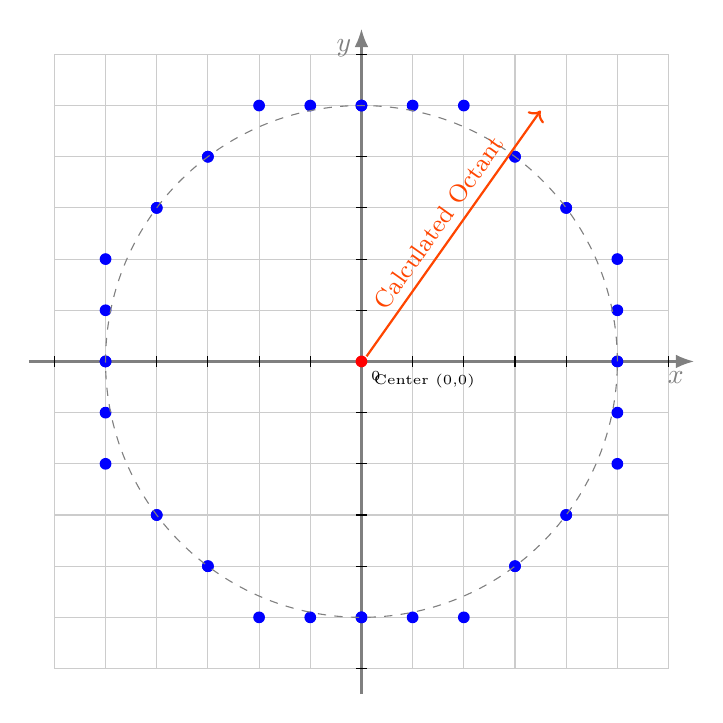
\begin{tikzpicture}[scale=0.65]
    % Grid
    \draw[gridline] (-6,-6) grid (6,6);

    % Axes
    \draw[axis] (-6.5,0) -- (6.5,0) node[below left] {$x$};
    \draw[axis] (0,-6.5) -- (0,6.5) node[below left] {$y$};

    % Origin Ticks
    \foreach \i in {-6,...,6} {
        \draw (\i, -0.1) -- (\i, 0.1);
        \draw (-0.1, \i) -- (0.1, \i);
    }
    \node[below right, font=\tiny] at (0,0) {0};

    % Center Point
    \node[centerpoint, label={[label distance=-1pt]below right:\tiny Center (0,0)}] at (0,0) {};

    % Calculated points and their symmetric counterparts
    % Points from calculation: (0,5), (1,5), (2,5), (3,4), (4,3)
    \drawCirclePoints{0}{5}
    \drawCirclePoints{1}{5}
    \drawCirclePoints{2}{5}
    \drawCirclePoints{3}{4}
    \drawCirclePoints{4}{3}

    % Dashed ideal circle
    \draw[dashedcircle] (0,0) circle (5);

    % Annotate one octant
    \draw[->, thick, OrangeRed] (0.1, 0.1) -- (3.5, 4.9) node[midway, above, sloped, font=\small] {Calculated Octant};
\end{tikzpicture}
\captionof{figure}{Plot of points for R=5 generated by Bresenham's algorithm, showing 8-way symmetry.}
\label{fig:tikz_circle}
\end{center}

\section{Code Implementations}

\subsection{C++ / OpenGL Snippet}
This snippet shows the core Bresenham logic. It assumes a function `drawPixel(x, y)` exists to plot a pixel relative to the circle center $(cx, cy)$ in an OpenGL context.

\begin{cppcode}
#include <GL/glut.h> // Or your preferred GL header

// Placeholder for actual pixel drawing function
void drawPixel(int x, int y) {
    // In a real scenario, you'd translate by (cx, cy)
    // and use appropriate OpenGL drawing commands.
    // Example: glVertex2i(x, y);
    glVertex2i(x, y);
}

// Function to draw all 8 symmetric points
void drawCirclePoints(int cx, int cy, int x, int y) {
    drawPixel(cx + x, cy + y);
    drawPixel(cx + y, cy + x);
    drawPixel(cx - x, cy + y);
    drawPixel(cx - y, cy + x);
    drawPixel(cx + x, cy - y);
    drawPixel(cx + y, cy - x);
    drawPixel(cx - x, cy - y);
    drawPixel(cx - y, cy - x);
}

// Bresenham's Circle Drawing Algorithm
void drawCircleBresenham(int cx, int cy, int r) {
    int x = 0;
    int y = r;
    int p = 3 - 2 * r; // Initial decision parameter

    // Start drawing points (typically within glBegin/glEnd)
    // glBegin(GL_POINTS); // Example

    // Draw the first set of points
    drawCirclePoints(cx, cy, x, y);

    // Calculate points for the second octant (0 to r/sqrt(2))
    while (x < y) {
        x++; // Always increment x
        if (p < 0) {
            // Move East
            p = p + 4 * x + 6;
        } else {
            // Move South-East
            y--;
            p = p + 4 * (x - y) + 10;
        }
        // Draw the calculated point and its symmetric counterparts
        drawCirclePoints(cx, cy, x, y);
    }

    // glEnd(); // Example
}

/*
// Example Usage in a GLUT display function:
void display() {
    glClear(GL_COLOR_BUFFER_BIT);
    glColor3f(0.0, 0.0, 1.0); // Set color to blue

    glBegin(GL_POINTS); // Begin drawing points
    drawCircleBresenham(0, 0, 50); // Draw circle at center (0,0) with radius 50
    glEnd(); // End drawing points

    glFlush();
}
*/
\end{cppcode}

\subsection{Python Snippet}
This Python code calculates the points in the second octant and provides a function to generate all symmetric points.

\begin{pythoncode}
import matplotlib.pyplot as plt

def bresenham_circle_octant(r):
    """
    Calculates points for the second octant (90 to 45 degrees)
    using Bresenham's circle algorithm.
    Starts at (0, r).
    """
    x = 0
    y = r
    p = 3 - 2 * r  # Initial decision parameter
    points = []

    # Add the starting point
    points.append((x, y))

    # Iterate until x >= y (end of the octant)
    while x < y:
        x += 1
        if p < 0:
            # Select point (x, y) - move East
            p = p + 4 * x + 6
        else:
            # Select point (x, y-1) - move South-East
            y -= 1
            p = p + 4 * (x - y) + 10

        points.append((x, y))

    return points

def get_symmetric_points(x, y):
    """Generates all 8 symmetric points for a given point (x, y)."""
    return [
        (x, y), (y, x), (-x, y), (-y, x),
        (x, -y), (y, -x), (-x, -y), (-y, -x)
    ]

def get_all_circle_points(cx, cy, r):
    """
    Generates all points for a circle centered at (cx, cy) with radius r.
    """
    octant_points = bresenham_circle_octant(r)
    all_points = set() # Use a set to avoid duplicates

    for x, y in octant_points:
        symmetric = get_symmetric_points(x, y)
        for sx, sy in symmetric:
            # Translate points relative to the center (cx, cy)
            all_points.add((cx + sx, cy + sy))

    return list(all_points)

# --- Example Usage ---
radius = 5
center_x = 0
center_y = 0

# Calculate points for the second octant
octant2_points = bresenham_circle_octant(radius)
print(f"Points in the second octant (R={radius}): {octant2_points}")

# Calculate all points for the circle
circle_points = get_all_circle_points(center_x, center_y, radius)
print(f"\nTotal unique points for the circle: {len(circle_points)}")
# print(f"All points: {sorted(list(circle_points))}") # Uncomment to see all points

# --- Optional: Plotting with Matplotlib ---
def plot_circle(points):
    if not points:
        print("No points to plot.")
        return

    x_coords, y_coords = zip(*points) # Unzip points into x and y lists

    plt.figure(figsize=(6, 6))
    plt.scatter(x_coords, y_coords, color='blue', s=10) # Plot points
    plt.axhline(0, color='grey', lw=0.5)
    plt.axvline(0, color='grey', lw=0.5)
    plt.grid(True, linestyle='--', alpha=0.6)
    plt.gca().set_aspect('equal', adjustable='box') # Ensure aspect ratio is equal
    plt.title(f"Bresenham's Circle Points (R={radius}, Center=({center_x},{center_y}))")
    plt.xlabel("X-axis")
    plt.ylabel("Y-axis")
    # Set limits slightly larger than radius
    lim = radius + 1
    plt.xlim(-lim, lim)
    plt.ylim(-lim, lim)
    plt.show()

# Plot the calculated points
# plot_circle(circle_points) # Requires matplotlib installed

\end{pythoncode}

\section{Summary}
\begin{tcolorbox}[
    colback=Green!10!white,
    colframe=ForestGreen!75!black,
    title=\faCheckCircle~ Key Takeaways,
    fonttitle=\bfseries\large
    ]
    \begin{itemize}
        \item Bresenham's Circle Algorithm provides an extremely efficient method for rasterizing circles using only integer operations.
        \item Its efficiency stems from incremental calculations based on a decision parameter and exploiting the inherent 8-way symmetry of circles.
        \item The algorithm calculates points for one octant, and symmetry rules generate the remaining points.
        \item It remains a fundamental algorithm in computer graphics for drawing circles and ellipses.
    \end{itemize}
\end{tcolorbox}

\end{document}
